%%%%%%%%%%%%%%%%%%%% author.tex %%%%%%%%%%%%%%%%%%%%%%%%%%%%%%%%%%%
%
% sample root file for your "contribution" to a contributed volume
%
% Use this file as a template for your own input.
%
%%%%%%%%%%%%%%%% Springer %%%%%%%%%%%%%%%%%%%%%%%%%%%%%%%%%%


% RECOMMENDED %%%%%%%%%%%%%%%%%%%%%%%%%%%%%%%%%%%%%%%%%%%%%%%%%%%
\documentclass[graybox]{svmult}

% choose options for [] as required from the list
% in the Reference Guide
\usepackage[margin=1.0in]{geometry}

\usepackage{subcaption}
\captionsetup{compatibility=false}
\usepackage{mathptmx}       % selects Times Roman as basic font
\usepackage{helvet}         % selects Helvetica as sans-serif font
\usepackage{courier}        % selects Courier as typewriter font
\usepackage{type1cm}        % activate if the above 3 fonts are
\usepackage{float}      % not available on your system
\usepackage{listings}
\usepackage{makeidx}         % allows index generation
\usepackage{graphicx}        % standard LaTeX graphics tool
%\graphicspath{ {/figures} }
\graphicspath{ {/Users/fonz/Documents/Projects/GTEx/plotting} }
\usepackage{multicol}        % used for the two-column index
\usepackage[bottom]{footmisc}% places footnotes at page bottom

% see the list of further useful packages
% in the Reference Guide

\makeindex             % used for the subject index
                       % please use the style svind.ist with
                       % your makeindex program

%%%%%%%%%%%%%%%%%%%%%%%%%%%%%%%%%%%%%%%%%%%%%%%%%%%%%%%%%%%%%%%%%%%%%%%%%%%%%%%%%%%%%%%%%

\begin{document}

\title*{First Year Report}
% Use \titlerunning{Short Title} for an abbreviated version of
% your contribution title if the original one is too long
\author{William Jones}
% Use \authorrunning{Short Title} for an abbreviated version of
% your contribution title if the original one is too long
\institute{William Jones \at Wellcome Trust Sanger Institute, \email{wj2@sanger.ac.uk}}
%
% Use the package "url.sty" to avoid
% problems with special characters
% used in your e-mail or web address
%
\maketitle

% Abstract - 200 words
%  Background - 1200 words
%  Aims - 200 words
%  Methods - 500 words
%  Results - 1000 words
%  Discussion - 900 words
%  Future work - 1000 words
%  Gantt chart outlining your future work plans
%  Tables - don’t use an excessive number
%  Figures - don’t use an excessive number
%  References


\abstract{200 words}
{Genome Wide Association Studies (GWAS) aim to understand the genetic basis of measurable traits. For effective and interpretable results, they require traits to be well-defined. Recently, imaging studies made available large datasets where samples are annotated with genetic and transcriptomic information. Owing to large variation within individual samples, it is difficult to extract well-defined features from images in order to investigate their genetic background. Existing work focuses on hand-crafted features, however we tackle this challenge with a different approach. We exploit neural networks, known for their ability to extract high-level concepts features from images and use the Genotype Tissue Expression (GTEx) Project high-resolution histology images annotated with bulk gene expression and genotype data.}

\section{Background 1200 words}
Biomedical images are used in the medical setting to predict onset of disease in autopsies. Diseases such as breast cancer, lung disease and heart disease. To what extent are the visual characteristics of biomedical images influenced by our our DNA, and the transcript levels within our tissues? To answer this question we use data from the The Genotype Tissue Expression (GTEx) project. This is a repository comprising genetics and bulk RNA expression data from multiple tissues and multiple donors. Early papers studying this data aimed to characterise gene expression variation and quantify eQTLs across different human tissues. At the time of analysis, the repository v6, consists of 449 genotyped individuals, and bulk RNA expression from 44 tissue types. Not every tissue type is available from each donor. A median of 15 tissues is given per individual, and a median of 155 samples per tissue type.

As of November 2016 - high resolution, histology Whole Side Tissue Image (WSTI) were made available for 34 tissue types. We investigated the samples of 10 well-known tissue types: Artery - Tibial, Brain - Cerebellum, Breast - Mammary Tissue, Heart - Left Ventricle, Liver, Lung, Ovary, Pancreas, Stomach and Testis.

There has already been work that looks to integrate these images with corresponding genetic data.  McCall et al \cite{complex-sources-of-variation} aim to use image data to reconcile the problem of unknown quantities of cell types within a tissue contributing to the bulk RNA expression of a sample. Within this analysis, they manually annotate the extent of pneumocyte hyperplasia of 114 lung images on a 0-3 scale, and find correlations between these annotations and expression levels of highly variable gene clusters. Although interesting, these image features needed to be handcrafted. This process is also labour intensive and expensive. Is it necessary to hand-craft these features?

Convolutional Neural networks were popularized by Karparthy et al in 2012 where they emphatically won the ILSVRC (ImageNet Large Scale Visual Recognition Challenge) with a top-5 test error rate of 15.3\% compared to a score of 26.2\% achieved by the second best entry. Since this point, they have become the most popular classification method in computer vision research. Importantly, they  are able to automatically learn feature representations of classes present in the input data. In 2014, Simonyan et al \cite{deep-inside-convolutional-networks} at the Visual Geometry Group in Oxford investigated the final layers of their ILSVRC2013 entry, VGG. They demonstrated that maximizing the activations of neurons deep within the network could generate features similar to the class labels that it was trained on - i.e. that discriminatory features from the images of the input data could be learned through the process of training the neural network to classify object classes.

From 2014 onwards, a new type of CNN architecture appeared - the Inception architecture, based on the ILSVRC2014 winning entry GoogLeNet. This allow neural networks to become deeper which being efficient with the number of parameters, and also learn more complex representations of imaging data.

Indirectly learning representations via training convolutional networks is not the only way to generate interesting feature representations. Lee et al \cite{scalable-unsupervised-learning} train convolutional deep belief network on datasets of natural faces, and demonstrate that early layers in the network serve as edge detectors, while middle and late neurons can progressively define complex image features like the contours of eyes, noses, and mouths, with the deepest able to fully the capture an approximate concept of a face.


\section{Aims 200 words}
In my first year, I aim to build upon these recent methods from computer vision research in order to answer the question of relating difficult datatypes in biomedical genetics. Using the GTEx image dataset, I aimed to:
\begin{enumerate}
 \item Retrain a convolutional neural network to classify tissue type based on pixel patches of varying sizes.
 \item Use the trained convolutional neural network as a features extractor to define a latent image representation.
 \item Understand and interpret what these different values in the latent representation mean.
 \item Understand the relationship of these high level representations to genotype and expression datasets.
\end{enumerate}
\label{sec:2}

\section{Methods 500 words}

\subsection{Tissue Classification}

\subsubsection{Neural Network architecture}

We defined two versions of Inceptionet-v3, a 220-layer Convolutional Neural Network pre-trained to distinguish everyday objects in images. The first neural network which we term raw InceptioNet, we used the weights that were generated from training the neural network on ImageNet, and which are able to classify 1000 different image classes. The second network, which we call retrained InceptioNet, we follow the common practice of adjusting the network architecture in order to fine-tune the network and repurpose it for a different task \cite{Gando et al.}. To finetune this network, we add a GlobalAveragePooling layer \cite{Lin et al} followed by a Dense layer a neural network, and a final softmax layer with 10 classification neurons.

\subsubsection{Data generation}

Much of the Whole Slide Tissues Image consisted of white empty space, with the area of tissue in question occupying a smaller area in the center. As such, we needed to define a patch sampling strategy that only extracted patches within the tissue boundary. In short, we needed to define the boundary between the tissue foreground and background, with the foreground consisting of the tissue area, and the background consisting of white-space. To do this, we applied Gaussian blurring to smooth edges contained with the image, and then applied the Otsu thresholding algorithm to segment the image into the tissue area foreground, and white background. Following this, for a given patch size $s$, we find the all the patch centers which lie within this tissue boundary. See Figure \ref{fig:extracting_tissue_patches}.

\subsubsection{Training the neural network}

When varying the size of patches, we re-scale all patches to be 299x299 pixels. This means that if we classifying a patch of size 4096, the size is drastically reduced to be 299x299. If the patch-size is 128x128, then we use bi-linear interpolation to resize the patch to be 299x299 pixels.

We fine-tuned our modified version of InceptioNet to classify square image patches into their originating tissue types. We sample 50 image patches within the tissue boundary from 100 images of 10 tissues, giving a total of 5000 patches per image class, with 50000 patches in total.

We use the categorical cross-entropy loss function with Stochastic Gradient Descent with learning rate 0.0001 and momentum = 0.9. We run the back-propagation algorithm to fine-tune the network in the following two steps:
\begin{enumerate}
 \item Update the final-layer weights for 10 epochs.
 \item Update the InceptionNet-v3 layer weights for 30 epochs.
\end{enumerate}


\subsection{Extracting Image level features}

Visual characteristics of the images are thought to be driven by levels of bulk RNA expression. We hypothesized that this relationship would be conserved when using the retrained neural network as a feature extractor, and that there would be a quantifiable relationship between these extracted features and transcript levels from bulk RNA expression and genotype data.  

Since our feature extractor was a convolutional neural network that which took as input square patches. Many square patch sizes fitted inside the boundary of the tissue slice, and the genetic data available only was representative of the entire image. As such, we needed a method to aggregate the features generated from multiple square patches of the same size, from patches located at different areas of the image into a single feature representative of the entire image. 

Concretely, we generated image level features from individual patches via the following steps.

\begin{enumerate}
 \item We segment the tissue slice into foreground and background using a Gaussian blur with kernel (51,51), followed by Otsu thresholding.
 \item Given a patch size, $s$, we find all patches of size s that lie within the tissue boundary. (See figure of segmenting tissues and finding patch centers)
 \item We pass each of these patches through the raw and retrained InceptioNet networks, at each to obtain an image feature vector of length 1024 for each patch.
 \item We take the aggregated image feature across all image patches. We compare aggregating via the mean and the median.
\end{enumerate}

Different image features manifest when looking at different scales. Therefore we investigated the aggregated image features generated through aggregating square patches of 6 different pixel widths. 128, 256, 512, 1024, 2048, and 4096. We chose these patch sizes because they represent the diversity of features at different resolutions. Within the patches with width 128 pixels we see individual cell nuclei and clusters of different cell types, whereas in large patch sizes we features characteristic of the entire image, for example colour or tissue shape. 

**Inline figure displaying patchsize 4096 and patchsize 128 from the same tissue**

We first visualized the features that were generated from each patch to assess which aggregation method would be most appropriate. Figure \ref{fig:patch_features_exploration} demonstrates the image feature activations for each patch for two different Lung tissues, with GTEx IDs GTEX-117YW-0526 and GTEX-117YX-1326. Although there exisits variation in individual features across patches in a tissue, there are strong drivers that are image specific, and different between each image. Furthermore, we see that although there is variation across patches for specific features, there exist global levels of activation present in all patches in the image, characteristic of an image level feature, rather than just a patch level features. These are indicated by faint horizontal bands, indicating consistent activation across patches for individual features. As such, we concluded that it would be reasonable to use and compare the median and mean activate across all patches in an image as the aggregation method.


\section{Results 1000 words}

\subsection{Tissue classification}

We compared the validation accuracy of using different patch sizes, and display them in Figure \ref{validation_accuracy_across_patchsize}. We achieved 81\% accuracy on held-out test data when using 128x128 patches in training and classification, and 94\% when using 4096x4096 image patches, demonstrating that neural networks trained on general tasks can be re-purposed for accurate biological image analysis. Despite the high levels of class ambiguity present at small pixel resolutions, the model is still able to achieve high accuracy. For larger patch sizes, global level features like average pixel intensity and tissue edge boundary seem to give accurate features to determine tissue class.

\subsection{Feature association}

\subsubsection{Exploratory Data analysis}

We choose Lung as the exemplary tissue in which to explore this method. We have a high number of samples from this tissue, and the image slices tend to be large. There was also a large amount of visual heterogeneity observed in the histopathology images across different samples. Figure \ref{fig:aggregated_features_across_samples} shows a heat maps of mean aggregated features, at a patch-size of $256$. We display 50 aggregated image feature values across the first 100 lung image samples, using retrained Inceptionet as the feature extractor in the top row, and raw Inceptionet on the bottom row. We see that there exists variation across sample when using both of these networks as features extractors, but that there exists a greater number of active features with retrained Inceptionet. We ask what drives the variation in later sections.

How much redundancy exists in these features? Do they capture independent visual characteristics? We consider image features generated from retrained Inceptionet features, mean aggregated at a patch-size of 256. In Figure \ref{fig:feature_crosscorrelation} we cross-correlate these features and perform hierarchical clustering understand their orthogonality and frequency of co-occurrence. Of the 1024 features, 380 were inactive across all samples. Therefore excluded these and proceeded using only the remaining 644. We see a large group of co-correlated features, but other groups along the diagonal that activate independently.

\subsubsection{Features Associations}

To understand whether drivers of variation in expression are related to drivers of variation in the image features, we took the first 10 expression principle components and the first 20 image feature principle components. We performed a pairwise correlation of these major axes of variation, which are displayed in figure \ref{fig:expression_PCs_vs_image_feature_PCs}. In the top left hand corner, we see that there exists a strong relationship between expression principle component $1$ and each of the image feature principle components $1$, $3$ and $6$. These have R score and p-values of $(-0.55, 4e-23)$, $(0.35, 4e-09)$, $(0.33, 2e-08)$ respectively. Furthermore, we see a relationship between image feature PC5 and expression PC2, image feature PC2 and expression PC6. These have R score and p-values of $(0.27, 9e06)$, $(-0.25, 3e-05) $ respectively.


It has been reported that technical factors drive variation in expression \cite{McCall et al. }, and so we investigated the source of this variation within samples. The GTEx dataset records conditions under which data was collected. For example, the total Ischemic time of a sample (SMTSISCH), RNA degradation number (SMRIN) and the code for the center where the sample was collected (SMCENTER). We collected the result of 51 technical features and correlate both the image feature PCs and the expression PCs with these technical factors in \ref{fig:expression_PCs_vs_TFs} and \ref{fig:image_feature_PCs_vs_TFs}. Interpreting \ref{fig:expression_PCs_vs_TFs},  We see that expression PC1 predominantly captures technical correlation, and is strongly related to the technical factors contained in \ref{tab:1}. The top 5 ordered correlations between the expression PCs and all technical factors all involve PC1.

Interpreting \ref{fig:expression_PCs_vs_image_feature_PCs}, we see that the same technical features correlate with image feature 1, albeit in a different order of p-values.

\subsubsection{Quantifying significant associations}

We wanted to investigate whether patch size influenced the core number of associations found between the generated image features and expression. To do this we calculated aggregated associations between the top 500 varying features across all patch sizes, and the top 1000 varying transcripts that have mean expression greater than $1$. We filter the both the image features and transcripts because most transcripts do not vary across samples and most image features are inactive. Figure \ref{fig:expression_means_and_stds} displays where the expression cutoff fall on the histograms of expression mean standard deviations respectively.

Figure \ref{fig:sign_pvalues_vary_patchsize} displays the results. We observe an interesting observation that across $3$ different false discovery thresholds there appears to be an optimum patch-size at $256x256$ pixels in order to find Bonferroni significant associations between the aggregated image features and individual transcripts. This is despite the fact that the network was  retrained to classify size 128x128 pixel patches. The number of associations steadily decreases up to a patch size of $4096$, where the number of associations reaches 0.

\subsubsection{Comparing Raw vs Retrained InceptioNet}

We assessed the degree to which the training process taught the network to detect tissue specific image features. In the same fashion as before, we extracted aggregated image features using raw InceptioNet. This network had been trained to differentiate natural images, but was not exposed to patches from histopathology tissue images. The final layer representation of raw Inceptionet was a vector of length 2048, therefore we filtered two sets of aggregated image features across all lung samples to include only the top 500 varying features across from the retrained and raw network respectively. This was an important step to ensure that we chose the same number of features for both cases. We quantified the number of Bonferroni significant associations across all patches sizes, and at 3 different false discovery rates. The results are displayed in Figure \ref{fig:sign_pvalues_raw_vs_retrained}. The associations from raw InceptioNet are displayed as the red line, and the associations from the retrained InceptionNet are displayed in the blue line. We notice that there are significantly more associations found at a patch size of 256 in retrained InceptioNet compared to that of raw InceptioNet. However for larger patch sizes, raw InceptioNet generates a greater number of significant associations, achieving a smaller maximum at patch size 512.

It might be that single features are strongly associated with the expression of very many genes. This is likely because gene expression is highly correlated amongst groups of genes with a similar biological function. Moreover, the extracted features demonstrate a high degree of correlation as shown by figure \ref{fig:feature_cross_correlation}. We investigate this question in the following sections.

\subsubsection{Comparing Aggregation methods}
In figure \ref{associations_mean_vs_median} we compare the aggregation methods, mean and median, used to combine features generated from individual patches across the extent of the tissue. We compare the Bonferonni significant associations between image features generated from Lung, at patch-size 256 at three different false discovery rates: $1e-2$, $1e-4$ and $1e-6$. As figure \ref{associations_mean_vs_median} shows, across each FDR the mean aggregate rate generates the greatest number of Bonferroni significant associations. This is true for all patch sizes considered, therefore we concluded that this was the best aggregation method out of the two options.

\subsubsection{Accounting for covarying transcripts and covarying features}

In figure \ref{fig:features_with_sign_transcripts} we count the number of features with Bonferroni significant associations to at least one transcripts. This gives us an indication of how active an image feature is at a particular patch size. We see in figure \ref{fig:features_with_sign_transcripts} a similar behaviour to when counting the raw numbers of associations. At a patch size of 256 we see the greatest number of features with at least 1 association to a transcript across all FDR thresholds, decreasing consistently for patch sizes greater than 256x256.

In figure \ref{transcripts_with_sign_features} we instead count the number of transcripts with Bonferroni significant associations to at least 1 feature. This gives us an indication of how many transcripts are connected to image features generated at each patch size. In this figure we see a slightly different behaviour than that of the previous two graphs. Here, we observe that the most number of associations is found at patch-size 512, as well as at the patch size of 256.


\subsection{Accounting for technical variation}

To account for technical variation, we performed the following steps:

We find large numbers of statistically significant genes across all patch-sizes. For example, patch size of 256 pixels we find 4710 statistically significant associations. (BH alpha < 0.01). We find that the greatest number of associations occurs at a patch-size of 256. We found that aggregating with the median results in a greater number of associations than when aggregating over the median for all patches sizes. We find a greater number of associations after fine-tuning Inceptionet, for a patch-size of 256, but a greater number of associations with raw Inceptionet when using patch sizes greater than this.
 
 
We assess how much variation is a cause of technical factors. Of the extracted 51 technical factors that describe sample conditions, some technical factors displayed extreme variation, therefore were discluded these. We take only the technical factors with standard devation < 100. This results in 29 technical factors. Examples include: RNA degradation (RIN) number, Exonic/Intronic mapping rates, and ischmeic time. We also investigate including $k$ of the first principle components as covariates. We used the $\lambda$ inflation parameter to assess p-value inflation.
 
We compare 3 models to disclude technical variation.
The first is to include them as a covariance parameter in linear mixed model (LMM), limix []. First, we did not include any technical covariates. We plot a QQplot of the pearsonr pvalues generated from the image features generated at a patch size of 256 with median aggregation in Figure \ref{fig:example_inflation_lung_256_mean}. We found these p-values to be highly inflated (lambda = 4.71), confirming that large factors of variation affected large groups of transcripts. 


We find 4323 significant associations (BH alpha=0.01). We found that including these 29 factors reduced the inflation to 2.57, and 1375 significant associations (BH alpha=0.01). We found that including the first 5 PCs reduced to inflation 1.57, and 107 significant associations (BH alpha=0.01). We found that including the first 5 PCs and the technical factors resulted in an inflation parameter of 1.71, and 77 significant associations (BH alpha=0.01).
The second was to compute the associations with the residuals after regressing out known variation. Regressing out the technical factors resulted in $\lambda$ = 1.63, and 29 significant associations (BG alpha = 0.01).  Regressing out the first 3 principle components resulted in $\lambda$ = 1.25, and 52 significant associations (BG alpha = 0.01). Including any more principle components resulted in a negative lambda value. Including both the technical factors and first 3 PCs resulted in a lambda of 0.85 and 2 significant associations (BG alpha = 0.01). Including both the technical factors and first 2 PCs resulted in a lambda of 0.98 and 7 significant associations (BG alpha = 0.01).
The third was to include the cross-correlation matrix computed from the expression matrix as a kinship matrix. This resulted in severely underinflated p-values with inflation parameter = 0.57.
 
We assessed that correcting for known variation regressing out the technical variation and 2 PCs resulting in appropriate levels of inflation. In Figure \ref{fig:corrected_scatterplots} we display the top 10 associations correcting for technical factors + 2 PCs for lung with patch-size of 256, we found the levels of expression from transcripts with gene IDs AGER, FCN3, and EPAS1 show a strong relation to the aggregated levels of many image features. It has not yet been reported in the literature that the levels of these genes give a visual effect. These transcripts did not display any correlation to known technical factors.

\subsubsection{Feature Interpretation}

We investigate which image features are associated to these 51 technical factors. In Figure \ref{fig:technical_factors_vs_image_features} we see many features highly correlated to the 5 core technical factors. Looking at the top 5 associations ordered by R**2 value, we see that image feature 796 displays a strong correlation with the technical factor SMTSISCH. (R -0.54 pvalue 1e-18).

We investigate what this features represents in figure \ref{fig:top5_bottom5_samples797}. Here we display the top and bottom 5 sample images of feature 797. We see a clear difference in the colour of the top 5 and bottom 5 samples. This colour change is strongly related to Ischemic time.

We investigate the function of other images features: for example in figure \ref{fig:top5_bottom5_samples351} we display the top and bottom 5 sample images of feature 351. This features picks up the porosity of the image, and is strongly linked to the technical factor RNA degradation (RIN number).



\section{Discussion 900 words}

We have successfully demonstrated that trained convolutional neural networks can be used to classify tissue type from individual square patches. We conclude that accuracy increases with increasing patch-size, suggesting that global level features like average pixel intensity and tissue edge boundary seem to give accurate features to determine tissue class.

Choosing Lung as a representative tissue, and using the trained convolutional neural network as a feature extractor, we generate aggregate image features for each sample. We find drivers of variation within the bulk RNA expression data for each tissue sample, and the image features we generated. Upon deeper investigation, we find that these drivers are largely technical. We compare strategies for correcting for this technical variation, and decide a strategy in which we include 29 of the 51 technical factors + the first 2PCs of the expression matrix as covariance in a linear mixed model. We observe that this corrects the QQplot, bringing the lambda parameter down from a value of 4.92 to 1.52. After correcting for the technical factors we report associations with individual gene transcripts that at this present point have not been known to be predicted from image information alone.

This work demonstrates that it is possible to gain information about gene expression using images alone. We find that variation was largely driven by technical factors, but that after comparing methods to regress out these external factors, we still find strong associations between image feature gene pairs that have previous gone unreported in the literature. 



\section{Future Work 1000 words}

Up until this point, this work has focussed on correcting for the high degree of technical noise plaguing both the expression and image dataset. One conclusion that can certainly be drawn from this work is that technical factors such as Ischemic time and Autolysis Score strongly impact the visual characteristic of image tissues, and these signals can be indirectly picked up by using trained neural networks as feature extractors. 

Despite the individual association signals that we report between image features and transcript, it is difficult to interpret what the image features capture. For image features that have a strong relationship with technical factors, they seem to only be capture trivial image features like colour and pixel intensity.

To improve the quality and variety of features that we can define, there are other classes of neural networks that can be used. For example, autoencoders are able to caputure image features and are trained in an unsupervised fashion. This is an approach that a competing group is currently pursuing, which I intent to compare with my approach. Furthermore, Generative Adverserial Networks (GANs) have recently become extremely impressive at defining latent image representations, and creating realistic images with them as input.

Since we were focussed on correcting for technical factors, we have neglected genotype. This is because we hypothesised that image features driven by technical factors would drown out the association signal to the genotype, which we already anticipate to be underpowered. A next step would be to investigate the relationship to the genotype of image features that show a relationship to transcripts after correcting for technica factors. 

Furthermore, the high levels features are not directly interpretable, neither via activation maximisation, saliency maps or ordering patches with respect to a feature. 

%\section{Gantt chart}

%\begin{figure}[H]
%\centering
%\includegraphics[width=0.9\textwidth]{Gantt}
%\caption{Gantt chart}
%\label{fig:gantt}
%\end{figure}


\section{Figures}

\begin{figure}[H]
\centering
\includegraphics[width=0.9\textwidth]{/FeatureExploration/extracting_tissue_patches}
\caption{In the left hand image, we illustrate how patch centers are formed within a tissue boundary. The blue dots represent patch centers that fit inside the tissue boundary. In the right hand image, we illustrate how the tissue is segmented into the tissue foreground and background by Gaussian blurring followed by Otsu thresholding.}
\label{fig:extracting_tissue_patches}
\end{figure}

\begin{figure}[H]
\centering
\includegraphics[width=0.5\textwidth]{/Classifier/validation_accuracy_across_patchsize}
\caption{This figure demonstrates the performance of our convolutional neural network in correctly classifying square tissue patches at different patch sizes. Each patch is resized to be 299x299 pixels. We see that at smaller resolutions, validation accuracy decreases but still achieves 81\% accuracy at patchsize 128x128.}
\label{fig:validation_accuracy_across_patchsize}
\end{figure}


\begin{figure}[H]
\centering
\includegraphics[width=0.7\textwidth]{/FeatureExploration/features_across_patches}
\caption{Image feature variation across patch from a single lung image}
\label{fig:features_across_patches}
\end{figure}


\begin{figure}[H]
\centering
\includegraphics[width=0.5\textwidth]{/FeatureExploration/aggregated_features_across_samples}
\caption{Figure showing 50 aggregated image feature values across 100 lung image samples. The top heatmap displays the image features from the retrained Inceptionet, and the bottom heatmap displays the image features from raw Inceptionet. More features are activated in retrained Inceptionet.}
\label{fig:aggregated_features_across_samples}
\end{figure}

\begin{figure}[H]
\centering
\includegraphics[width=0.5\textwidth]{/FeatureExploration/feature_crosscorrelation}
\caption{Hierachical clustering performed on aggregated image features with non-zero standard deviation.}
\label{fig:feature_cross_correlation}
\end{figure}

\begin{figure}[H]
\centering
\includegraphics[width=0.6\textwidth]{/PCAFeatureAssociations/expression_PCs_vs_image_feature_PCs}
\caption{Pairwise pearsonr correlation analysis between image feature PCs and expression PCs describing 95\% of the variation of the respective datasets. A strong relationship exists between expression PC 1 and image feature PC1.}
\label{fig:expression_PCs_vs_image_feature_PCs}
\end{figure}


\begin{figure}[H]
\centering
\includegraphics[width=0.4\textwidth]{/PCAFeatureAssociations/expression_PCs_vs_TFs}
\caption{Pairwise pearsonr correlation analysis between 51 technical factors and the first 10 expression PCs. A strong relationship exists between expression PC1 and 5 technical factors. This is described in more detail within Table \ref{tab:expression_pcs_and_tfs} }
\label{fig:expression_PCs_vs_TFs}
\end{figure}

\begin{figure}[H]
\centering
\includegraphics[width=0.4\textwidth]{/PCAFeatureAssociations/image_feature_PCs_vs_TFs}
\caption{Pairwise pearsonr correlation analysis between 51 technical factors and the first 10 image feature principle components. A strong relationship exists between image features PC1 and 5 technical factors. This is described in more detail within Table \ref{tab:image_feature_pcs_and_tfs} }
\label{fig:technical_factors_vs_pca_feature}
\end{figure}

\begin{figure}[H]
\centering
\includegraphics[width=0.6\textwidth]{/FeatureExploration/expression_means_and_stds}
\caption{The left hand figure displays a histogram of mean expression of transcripts across the lung samples. The red cutoff line indicates the proportion of transcripts that have mean expression greater than 1. The right hand figure displays a histogram of transcript standard deviations across the lung samples that have been filtered to have mean expression greater than 1. The right hand side of the red cutoff line indicate the 1000 most varying transcripts.}
\label{fig:expression_means_and_stds}
\end{figure}

\begin{figure}[H]
\centering
\includegraphics[width=0.7\textwidth]{/RawFeatureAssociations/raw_associations_across_patchsizes}
\caption{A graph showing the relationship between raw number of Bonferroni significant associations for 3 different FDRs: 1-e2, 1-e4 and 1-e6. We see that at a patch size of 256x256 we find the greater number of associations across all FDRs.}
\label{fig:raw_associations_across_patchsizes}
\end{figure}

\begin{figure}[H]
\centering
\includegraphics[width=0.7\textwidth]{/RawFeatureAssociations/associations_raw_vs_retrained}
\caption{A graph showing the relationship between raw number of Bonferroni significant associations for 3 different FDRs: 1-e2, 1-e4 and 1-e6. We see that at a patch size of 256x256 we find the greater number of associations across all FDRs.}
\label{fig:associations_raw_vs_retrained}
\end{figure}

\begin{figure}[H]
\centering
\includegraphics[width=0.7\textwidth]{/RawFeatureAssociations/associations_mean_vs_median}
\caption{A graph showing the relationship between raw number of Bonferroni significant associations for 3 different FDRs: 1-e2, 1-e4 and 1-e6. We see that at a patch size of 256x256 we find the greater number of associations across all FDRs.}
\label{fig:associations_mean_vs_median}
\end{figure}


%\begin{figure}[H]
%\begin{subfigure}{0.5\textwidth}
%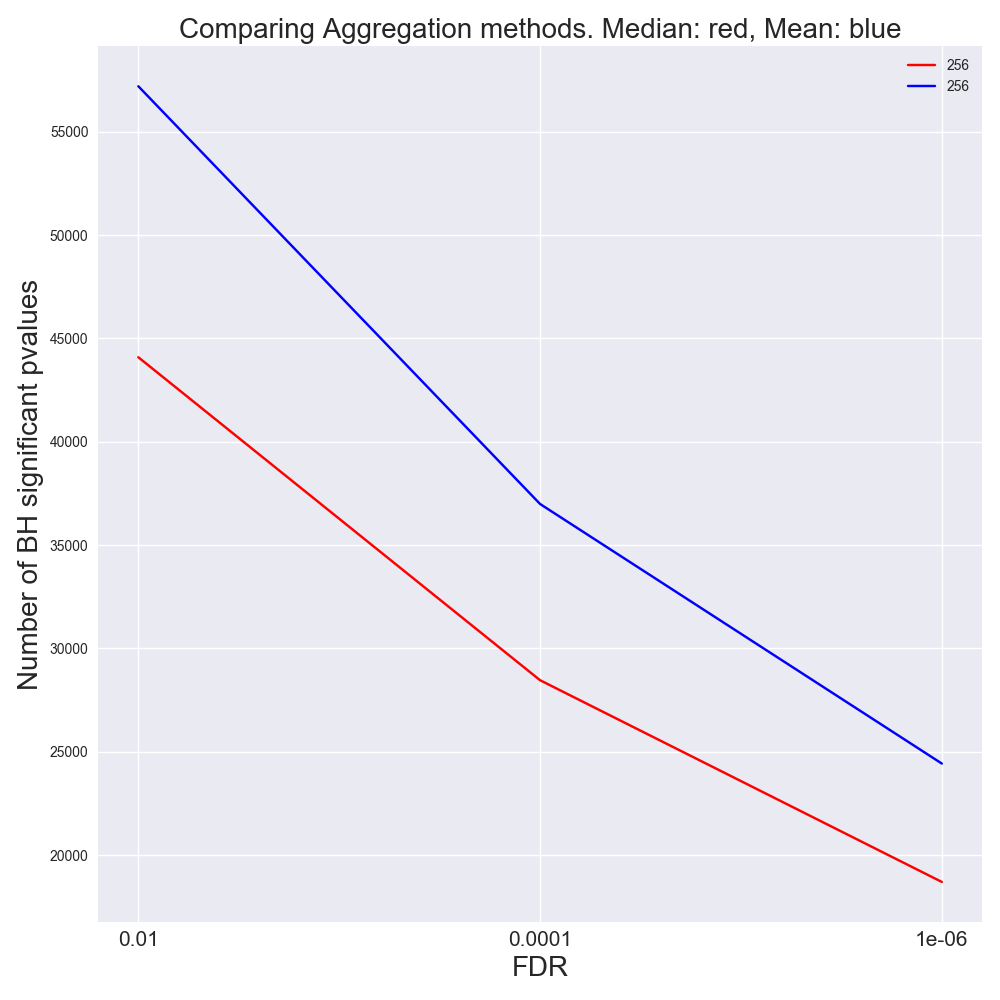
\includegraphics[width=1\linewidth, height=6cm]{sign_pvalues_mean_vs_median} 
%\caption{}
%\label{fig:sign_pvalues_mean_vs_median}
%\end{subfigure}
%\begin{subfigure}{0.5\textwidth}
%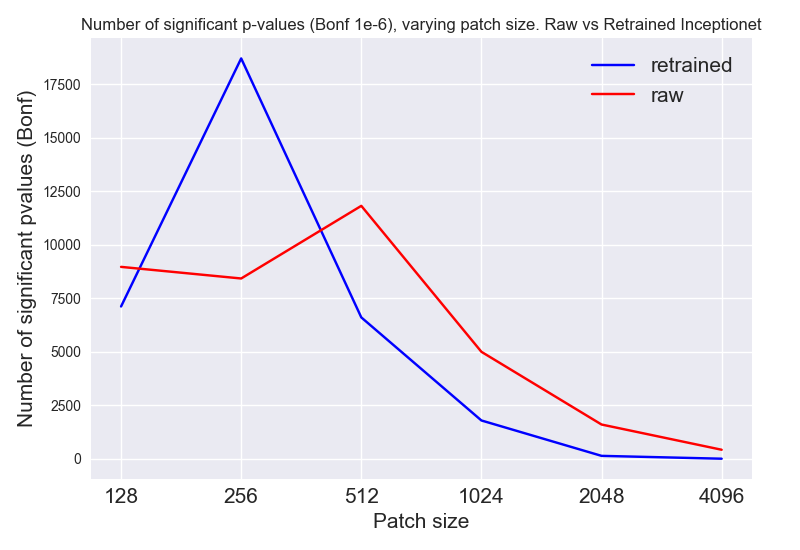
\includegraphics[width=1\linewidth, height=6cm]{sign_pvalues_raw_vs_retrained}
%\caption{}
%\label{fig:sign_pvalues_raw_vs_retrained}
%\end{subfigure}

%\caption{}
%\label{fig:sign_pvalues_mean_vs_median_raw_vs_retrained}
%\end{figure}

\begin{figure}[H]
\centering
\includegraphics[width=0.4\textwidth]{/RawFeatureAssociations/features_with_significant_transcripts} 
\caption{Number of features with a significant expression association}
\label{fig:features_with_significant_transcripts}
\end{figure}

\begin{figure}[H]
\centering
\includegraphics[width=0.4\textwidth]{/RawFeatureAssociations/transcripts_with_significant_features}
\caption{Number of transcripts with significant feature association}
\label{fig:transcripts_with_significant_features}
\end{figure}

%\begin{figure}[H]
%\centering
%\includegraphics[width=0.7\textwidth]{top5_bottom5_samples351}
%\caption{The top row displays the top 5 samples for aggregated feature 351, the bottom row displays the bottom 5 samples. Notice the stark difference in colour.}
%\label{fig:top5_bottom5_samples351}
%\end{figure}

%\begin{figure}[H]
%\centering
%\includegraphics[width=0.7\textwidth]{top5_bottom5_samples797}
%\caption{The top row displays the top 5 samples for aggregated feature 351, the bottom row displays the bottom 5 samples. Notice the stark difference in porosity.}
%\label{fig:top5_bottom5_samples797}
%\end{figure}


%\begin{figure}[H]
%\centering
%\includegraphics[width=0.7\textwidth]{example_inflation_lung_256_mean}
%\caption{}
%\label{fig:example_inflation_lung_256_mean}
%\end{figure}


%\begin{figure}[H]
%\centering
%\includegraphics[width=0.7\textwidth]{corrected_pvalues_qqplot}
%\caption{}
%\label{fig:corrected_pvalues_qqplot}
%\end{figure}

%\begin{figure}[H]
%\centering
%\includegraphics[width=0.7\textwidth]{corrected_scatterplots}
%\caption{}
%\label{fig:corrected_scatterplots}
%\end{figure}

\section{Tables}

\begin{table}
\caption{Top 5 R\textsuperscript{2} associations between Expression PCs and technical factors}
\label{tab:expression_pcs_and_tfs}       % Give a unique label
%
% Follow this input for your own table layout

\begin{tabular}{p{1cm}p{2.4cm}p{8cm}p{1cm}p{1cm}}
\hline\noalign{\smallskip}
 PC & Technical factor & Description & R score & p-value  \\
\noalign{\smallskip}\svhline\noalign{\smallskip}
1 & SMTSISCH & Total Ischemic time for a sample in 4 hour intervals & 0.78 & 3e-48\\
1 & SMNTRNRT & Intronic Rate: The fraction of reads that map within introns & 0.77 & 4e-45\\
1 & SMNTRNRT & Exonic Rate: The fraction of reads that map within exons & -0.73 & 3e39 \\
1 & SMRIN & RIN Number (RNA degradation) & -0.61 & 2e-24 \\
1 & SMATSSCR & Autolysis Score & 0.46 & 3e-13 \\
\noalign{\smallskip}\hline\noalign{\smallskip}
\end{tabular}
% $^a$ Table foot note (with superscript)
\end{table}

\begin{table}
\caption{Top 5 R\textsuperscript{2} associations between Expression PCs and technical factors}
\label{tab:image_feature_pcs_and_tfs}       % Give a unique label

\begin{tabular}{p{1cm}p{2.4cm}p{8cm}p{1cm}p{1cm}}
\hline\noalign{\smallskip}
PC & Technical factor & Description & R score & p-value  \\
\noalign{\smallskip}\svhline\noalign{\smallskip}
1 & SMRIN & RIN Number (RNA degradation) & 0.49 & 2e-15\\
1 & SMTSISCH & Total Ischemic time for a sample in 4 hour intervals, & 0.77 & 4e-45\\
1 & SMATSSCR & Autolysis Score & -0.42 & 4e-11 \\
1 & SMNTRNRT & Intronic Rate: The fraction of reads that map within introns & -0.41 & 8e-11 \\
1 & SMEXNCRT & Exonic Rate: The fraction of reads that map within exons & 0.37 & 5e-09 \\
\noalign{\smallskip}\hline\noalign{\smallskip}
\end{tabular}
% $^a$ Table foot note (with superscript)
\end{table}



%%%%%%%%%%%%%%%%%%%%%%%%% referenc.tex %%%%%%%%%%%%%%%%%%%%%%%%%%%%%%
% sample references
% %
% Use this file as a template for your own input.
%
%%%%%%%%%%%%%%%%%%%%%%%% Springer-Verlag %%%%%%%%%%%%%%%%%%%%%%%%%%
%


\begin{thebibliography}{99.}

\bibitem{histology-classification-lung-cancer} Lamb D. Histological classification of lung cancer. Thorax. 1984;39(3):161-165.

\bibitem{detecting-cancer-metastases} Yun Liu \& Krishna Gadepalli (2017) Detecting Cancer Metastases on Gigapixel Pathology Images http://arxiv.org/abs/1703.02442v2

\bibitem{gene-expression-parkinsons} Lewis, P. A., \& Cookson, M. R. (2012). Gene expression in the Parkinson's disease brain. Brain Research Bulletin, 88(4), 302?312. http://doi.org/10.1016/j.brainresbull.2011.11.016

\bibitem{what-is-complex-about-complex-disorders} Mitchell, K. J. (2012). What is complex about complex disorders? Genome Biology, 13(1), 237. http://doi.org/10.1186/gb-2012-13-1-237

\bibitem{GTEx-project} Lonsdale, J., Thomas, J., Salvatore, M., Phillips, R., Lo, E., Shad, S., et al. (2013). The Genotype-Tissue Expression (GTEx) project. Nature Genetics, 45(6), 580?585. http://doi.org/10.1038/ng.2653

\bibitem{GTEx-histology} GTEx Image Viewer https://brd.nci.nih.gov/brd/image-search/searchhome

\bibitem{surfectant-dysfunction} Susan E. Wert Jeffrey A. Whitsett (2009) Genetic Disorders of Surfactant Dysfunction http://journals.sagepub.com/doi/10.2350/09-01-0586.1

\bibitem{complex-sources-of-variation} McCall, M. N., Illei, P. B., \& Halushka, M. K. (2016). Complex Sources of Variation in Tissue Expression Data: Analysis of the GTEx Lung Transcriptome. The American Journal of Human Genetics, 99(3), 624��635. http://doi.org/10.1016/j.ajhg.2016.07.007

%\bibitem{scalable-unsupervised-learning} Lee, H., Grosse, R., Ranganath, R., \& Ng, A. Y. (2009). Convolutional deep belief networks for scalable unsupervised learning of hierarchical representations. Proceedings of the 26th annual pp.609616�� ACM. http://doi.org/10.1145/1553374.1553453
%



%
%\bibitem{autoencoders-unsupervised-learning-and-deep-architectures} Baldi, P. (2012). Autoencoders, unsupervised learning, and deep architectures. Presented at the Proceedings of ICML Workshop on Unsupervised and ?.
%
\bibitem{shapiro-computer-vision} Shapiro, L. G. \& Stockman, G. C: "Computer Vision", page 137, 150. Prentice Hall, 2001
%
\bibitem{otsu-method} Otsu, N. (1979). A Threshold Selection Method from Gray-Level Histograms. IEEE Transactions on Systems, Man, and Cybernetics, 9(1), 62?66. http://doi.org/10.1109/TSMC.1979.4310076

\bibitem{network-in-network} Lin, M., Chen, Q., \& Yan, S. (2013, December 16). Network In Network. arXiv.org.


\bibitem{inception} Christian Szegedy, Vincent Vanhoucke, Sergey Ioffe, Jonathon Shlens, Zbigniew Wojna (2 Dec 2015). Rethinking the Inception Architecture for Computer Vision https://arxiv.org/abs/1512.00567
%
\bibitem{keras} Keras Chollet, Fran\c{c}ois and others, https://github.com/fchollet/keras
%
\bibitem{openslide} Goode. (2012). OpenSlide: A vendor-neutral software foundation for digital pathology. Journal of Pathology Informatics, 4(1), 27. http://doi.org/10.4103/2153-3539.119005
%
%\bibitem{generative-adverserial-networks} Goodfellow, I., Pouget-Abadie, J., Mirza, M., Xu, B., Warde-Farley, D., Ozair, S., et al. (2014). Generative Adversarial Nets. Advances in Neural ?, 2672?2680.
%
%\bibitem{gans-biological-image-synthesis} Osokin, A., Chessel, A., Salas, R. E. C., \& Vaggi, F. (2017, August 15). GANs for Biological Image Synthesis. arXiv.org.
%
%\bibitem{variational-autoencoders} Kingma, D. P., \& Welling, M. (2013, December 20). Auto-Encoding Variational Bayes. arXiv.org.
%
%\bibitem{fully-convolutional-networks} Long, J., Shelhamer, E., \& Darrell, T. (2015). Fully Convolutional Networks for Semantic Segmentation. Proceedings of the IEEE ?, 3431?3440.
%
%\bibitem{sparse-autoencoders} Hou, L., Nguyen, V., Samaras, D., Kurc, T. M., Gao, Y., Zhao, T., \& Saltz, J. H. (2017, April 3). Sparse Autoencoder for Unsupervised Nucleus Detection and Representation in Histopathology Images. arXiv.org.
%
%\bibitem{segmenting-classifying-epithelial} Xu, J., Luo, X., Wang, G., Gilmore, H., \& Madabhushi, A. (2016). A Deep Convolutional Neural Network for segmenting and classifying epithelial and stromal regions in histopathological images. Neurocomputing, 191, 214?223. http://doi.org/10.1016/j.neucom.2016.01.034
%
%\bibitem{mendelian-randomization} Smith, G. D., \& Ebrahim, S. (2008). Mendelian Randomization: Genetic Variants as Instruments for Strengthening Causal Inference in Observational Studies.
%
%\bibitem{hipsci-project} Streeter, I., Harrison, P. W., Faulconbridge, A., Flicek, P., Parkinson, H., \& Clarke, L. (2017). The human-induced pluripotent stem cell initiative?data resources for cellular genetics. Nucleic Acids Research, 45(D1), D691?D697. http://doi.org/10.1093/nar/gkw928

\end{thebibliography}




\end{document}
